% % % % % % % % % % % % % % % % % % % % % % % % % % % % % % % % % % % % % % % % % % % %
%                                                                                     %
% Short Sectioned Assignment LaTeX Template Version 1.0 (5/5/12)                      %
% This template has been downloaded from: http://www.LaTeXTemplates.com               %
%                                                                                     %
% Original author:  Frits Wenneker (http://www.howtotex.com)                          %
%                                                                                     %
% Modified by: Fco Javier Sueza Rodríguez (fcosueza@disroot.org)                      %
%                                                                                     %
% Changes:                                                                            %
%	    - Custom Chapters, Sections and Subsections (titlesec package)                %
%           - Document type scrbook (oneside)                                         %
%           - Use babel-lang-spanish package and marvosym                             %
%           - Use hyperref, enumitem, tcolorbox and glossaries packages               %
%           - Use Time New Roman (mathptmx), Helvetic and Courier fonts               %
%                                                                                     %
% License: CC BY-NC-SA 3.0 (http://creativecommons.org/licenses/by-nc-sa/3.0/)        %
%                                                                                     %
% % % % % % % % % % % % % % % % % % % % % % % % % % % % % % % % % % % % % % % % % % % %

%-----------------------------------------------%
%	              Packages                  %
%-----------------------------------------------%

\documentclass[paper=a4, fontsize=11pt, oneside]{scrbook}

% ---- Text Input/Output ----- %

\usepackage[T1]{fontenc}
\usepackage[utf8]{inputenc}
\usepackage{mathptmx}
\usepackage[scaled=.92]{helvet}
\usepackage{courier}
\usepackage[indent=12pt]{parskip}

\usepackage{geometry}
\geometry{verbose,tmargin=3cm,bmargin=3cm,lmargin=2.6cm,rmargin=2.6cm}

% ---- Language ----- %

\usepackage[spanish]{babel}
\usepackage{marvosym}

% ---- Another packages ---- %

\usepackage{amsmath,amsfonts,amsthm}
\usepackage{graphics,graphicx}
\usepackage{titlesec}
\usepackage{fancyhdr}
\usepackage{tcolorbox}
\usepackage{hyperref}
\usepackage{enumitem}
\usepackage[automake]{glossaries}

%--------------------------------------------------------------------%
%                      Customizing Document                          %
%--------------------------------------------------------------------%


% ----------- Custom Chapters, Sections and Subsections -------------- %

\titleformat{\chapter}[display]
			{\bfseries\Huge}
			{Tema \ \thechapter} {0.5ex}
			{\vspace{1ex}\centering}

\titleformat{\section}[hang]
			{\bfseries\Large}
			{\thesection}{0.5em}{}

\titleformat{\subsection}[hang]
			{\bfseries\large}
			{\thesubsection}{0.5em}{}

\titleformat{\subsubsection}[hang]
			{\bfseries\large}
			{\thesubsubsection}{0.5em}{}

\hypersetup{
    colorlinks=true,
    linkcolor=black,
    urlcolor=magenta
}

% ------------------- Custom heaaders and footers ------------------- %

\pagestyle{fancyplain}

\fancyhead[]{}
\fancyfoot[L]{}
\fancyfoot[C]{}
\fancyfoot[R]{\thepage}

\renewcommand{\headrulewidth}{0pt} % Remove header underlines
\renewcommand{\footrulewidth}{0pt} % Remove footer underlines

\setlength{\headheight}{13.6pt} % Customize the height of the header

% --------- Numbering equations, figures and tables ----------------- %

\numberwithin{equation}{section} % Number equations within sections
\numberwithin{figure}{section} % Number figures within sections
\numberwithin{table}{section} % Number tables within sections

% ------------------------ New Commands ----------------------------- %

\newcommand{\horrule}[1]{\rule{\linewidth}{#1}} % Create horizontal rule command


%----------------------------------------------------------------------------------------
%	TÍTULO Y DATOS DEL ALUMNO
%----------------------------------------------------------------------------------------

\title{
\normalfont \normalsize
\textsc{{\bfseries Curso 2022-2023} \\ Ciclo Superior de Desarrollo de Aplicaciones Web \\ IES Aguadulce} \\ [25pt]
\horrule{0.5pt} \\[0.4cm]
\huge Sistemas Informáticos \\
\horrule{0.5pt} \\[0.4cm]
}

\author{Francisco Javier Sueza Rodríguez}
\date{\normalsize\today}

%----------------------------------------------------------------------------------------
%                                     DOCUMENTO
%----------------------------------------------------------------------------------------
\makeglossaries
\loadglsentries{glossary.tex}

\begin{document}

\maketitle

\newpage

\tableofcontents

\listoffigures

%\listoftables

\newpage

\chapter{Hardware de un Sistemas Informático}
En esta primera unidad de la asignatura ``\textbf{Sistemas Informáticos}, vamos a ver los conceptos básicos de sobre los sistemas informáticos, centrándonos principalmente en el apartado del hardware de un sistema informático. Así, veremos cuales son los diferentes componente hardware (o físicos) de un computador, así como la información necesaria para su ensamblaje y puesta en marcha.

También veremos diferentes tipos de clasificaciones de los ordenadores, incluyendo los ordenadores personales, así como otra información útil que podremos encontrar en los diferentes anexos que se incluyen al final de esta unidad.

\section{Sistema Informático}
La \textbf{informática} es la ciencia que se encarga de estudiar todo lo relacionado con los sistemas informáticos, incluyendo los temas relativos a su arquitectura y fabricación, hasta los temas referidos al almacenamiento y organización de la información, sin olvidar la creación y uso de software, o la formación del personal informático. Para ello, se apoya en múltiples disciplinas como las matemáticas, física, electrónica, etc...

Un \textbf{sistema informático} es el conjunto de \textbf{elementos físicos} (hardware) y \textbf{elementos lógicos} (software), interconectados entre sí, destinados a gestionar el \textbf{tratamiento automático de la información}, entendiendo por esto, su almacenamiento, transmisión, organización y/o procesamiento.

Se incluye, como parte fundamental de un sistema informático, al \textbf{conjunto de personas} que lo \textbf{utiliza}, ya sean usuario, administradores, programadores, etc... El elemento humano es un \textbf{componente imprescindible}, ya que los sistemas informáticos son creados, desarrollados y utilizados por humanos para su propio provecho.

En sistema informáticos siempre debemos distinguir entre hardware y software:

\begin{itemize}
    \item \textbf{Hardware}: son todos los elementos físicos que forman parte de un ordenador, es decir, teclado, ratón, placa base, monitor, memoria, disco duro, cables, etc... Es la ``maquinaria'' necesaria utilizada para el tratamiento de la información.
    \item \textbf{Software}: es el elemento lógico e ``intangible'' de un sistema informático. Se compone de un conjunto de programas y datos que permiten manejar el hardware, controlando y coordinando su funcionamiento para que pueda realizar las tareas esperadas. Esta compuesto principalmente de dos elementos:
    \begin{itemize}
        \item \textbf{Programas}: están formados por un conjunto de órdenes o instrucciones que se utilizan para procesador los datos que se introducen como información. Son necesarios para la gestión y el control de los equipos y los trabajos de los usuarios.
        \item \textbf{Datos}: son la información que los programas deben procesar, utilizando para esto diferentes elementos hardware que componen el sistema informático. Son, en definitiva, la razón de ser el sistema informático.
    \end{itemize}
\end{itemize}

Los \textbf{sistemas informáticos} han \textbf{evolucionado}. En un principio todos sus componentes, físicos, lógicos y humanos, estaban localizados en el mismo lugar, pero actualmente están formados por subsistemas que se interconectan a través de la red, que pueden llegar a estar a miles de kilómetros de distancia entre sí, integrando sistemas complejos de procesamiento de la información. Estos subsistemas a si vez pueden estar compuestos por un superodenador, un ordenador personal, redes locales de ordenadores o por una combinación de todos ellos, siendo el sistema informático más simple el formado por un ordenador y un usuario que ejecuta programas en él.

Un \textbf{ordenador} se define como una máquina electrónica, con algunas partes mecánicas, compuesta por al menos, una unidad de proceso, y por equipos periféricos, controlada por programas que deben estar almacenados en su memoria central, destinada al tratamiento automático de la información que le es suministrada. Es una máquina de propósito general ya que puede realizar gran variedad de trabajos y a gran velocidad.

En el \textit{Anexo A.1}, podrás encontrar más información sobre la clasificación de los ordenadores.

\section{Arquitectura Hardware: Componentes Funcionales}
Un computador esta compuesto por una seria de sistemas y subsistemas hardware, que cooperando entre sí, permiten a este llevar a cabo su función, procesando la información que recibe y emitiendo los resultados de este procesado.  En la siguiente figura vemos un esquema de estos subsistemas.

\begin{figure}[ht]
    \centering
    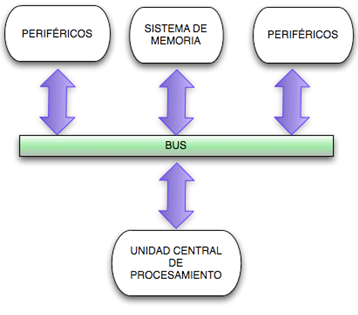
\includegraphics[scale=0.90]{arquitectura-computador.png}
    \caption{Subsistemas de la arquitectura de un computador}
\end{figure}


Como vemos en la imagen, hay tres subsistemas principales, que son los siguientes:

\begin{itemize}
    \item \textbf{Unidad Central de Proceso} (CPU): es el sistemas básico más importante, encargado de coordinar a los demás subsistemas, extraer secuencialmente las instrucciones de la memoria principal para procesarlas y ejecutarlas.
    \item \textbf{Sistemas de Memoria}: su función básica es la de almacenar las instrucciones que se van a procesar posteriormente, los datos y los resultados que sean necesarios.
    \item \textbf{Periféricos}: se dividen en periféricos de entrada y de salida, según la dirección del flujo de información. Ambos sistemas se encargan de la comunicación con el exterior, es decir, con el usuario u otros sistemas.
\end{itemize}

Además de estos tres subsistemas, debemos de hablar de \textbf{bus de sistema}, que es el medio físico encargado de transmitir la información entre los diferentes subsistemas.

En la actualidad, la arquitectura empleada es la fabricación de computadores es la \textbf{arquitectura Von Neumann}. Esta arquitectura de computadoras ésta basada en la descrita en 1945 por el matemático y físico \textbf{John Von Neumann}. En la siguiente imagen podemos ver un esquema de la arquitectura Von Neumann.

\begin{figure}[ht]
    \centering
    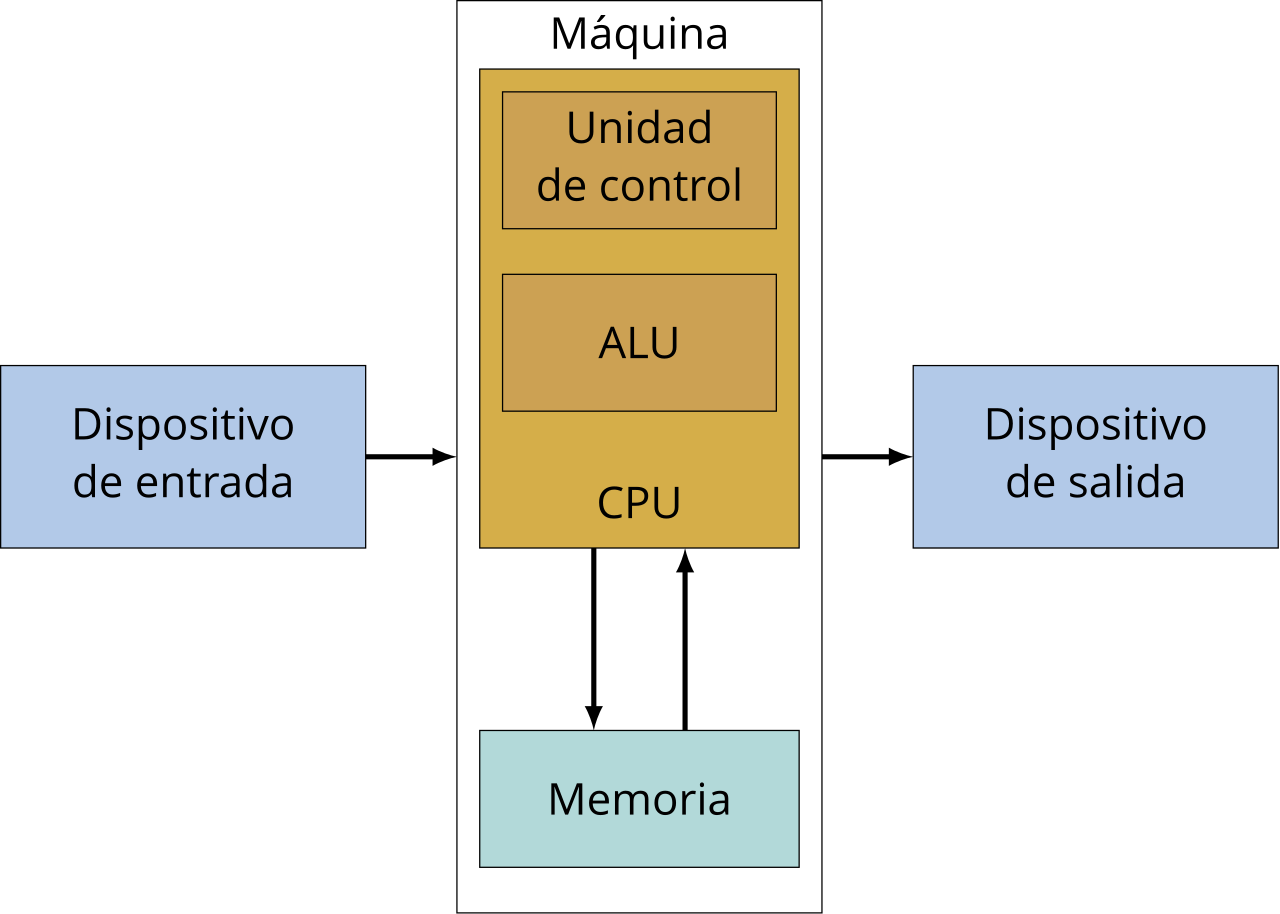
\includegraphics[scale=0.25]{von-neumann.png}
    \caption{Arquitectura Von Neumann}
\end{figure}

Como vemos es igual a la que hemos descrito en este punto. Podemos observar como la \textbf{CPU} contiene dos unidades, la \textbf{unidad de control} y la \textbf{ALU} o \textbf{unidad Aritmético-Lógica}, las cuales veremos con más detalle en la siguiente sección.

Si queremos saber más sobre esta arquitectura, lo cual recomiendo encarecidamente, podemos visitar \href{https://es.wikipedia.org/wiki/Arquitectura_de_Von_Neumann}{la entrada en Wikipedia} de la arquitectura Von Neumann.

\subsection{Componentes Principales (CPU, RAM, E/S, ...)}
La \textbf{Unidad Central de Proceso} es el componente que podría definirse como el ``cerebro'' del computador, ya que es la encargada de controlar, dirigir y coordinar todas las operaciones que realiza el ordenador.

Para que la CPU pueda ejecutar un \textbf{\gls{programa}} es necesario que éste se guarde en su memoria principal, desde donde se van extrayendo en secuencia cada una de sus instrucciones, analizándolas y emitiendo las órdenes necesarias al resto de componentes que deban intervenir para completar su ejecución.

La CPU esta integrada en el Procesador Central o microprocesador y acompañada de una pequeña cantidad de \textbf{\gls{registros}} de memoria necesarios para su funcionamiento.

Dentro del Microprocesador, y como parte integrante de la \textbf{CPU}, existen dos unidades, como ya vimos en el apartado anterior sobre la arquitectura Von Neumann. Esta unidades son:

\begin{itemize}
    \item \textbf{Unidad de Control}: se encarga de ejecutar los programas, controlando su secuencia, interpretando y ejecutando las instrucciones. Se encarga también de controlar al resto de componentes, como periféricos, memoria, etc.., según vayan necesitando las instrucciones.
    \item \textbf{Unidad Aritmético-Lógica} o \textbf{ALU}: se encarga de realiza los cálculos matemáticos y lógicos necesarios para su funcionamiento.
\end{itemize}

La memoria principal, conocida como \textbf{RAM} (Random Access Memory), es la encargada de almacenar los datos e instrucciones de los programas que deben ejecutarse, así como toda la información que el sistema necesita para su funcionamiento. Esta constituida por un \textbf{conjunto de registros} capaces de retener información en su interior mientras el ordenador esta en funcionamiento. Cuando el ordenador se apaga, se pierde su contenido, por lo que esta memoria es de tipo \textbf{\gls{volatil}}.

Los \textbf{sistemas de Entrada y Salida} son circuitos electrónicos que permiten el intercambio de información entre la CPU y los periféricos. Las unidades de entrada y salida se usan para cargar programas y datos en memoria principal desde los periféricos de entrada, y las unidades de salida para mostrar los resultados de las operaciones realizadas a través de periféricos de salida.

Los \textbf{buses del sistema} son el conjunto de circuitos eléctricos que conectan la CPU con el resto de componentes para comunicarse entre sí. Cada bus es un conjunto de cables de un circuito integrado que permite la transmisión de información de forma paralela. Podemos encontrar tres tipos diferentes de buses:

\begin{itemize}
    \item \textbf{Bus de Instrucciones y Datos}: se utilizan para trasladar tanto instrucciones como datos desde la memoria RAM al resto de componentes del computador y viceversa.
    \item \textbf{Bus de Control}: bus que se encarga de trasmitir las instrucciones desde la CPU al resto de unidades y recibe de ellas señales indicando su estado.
    \item \textbf{Bus de Direcciones}: se encarga de transmitir las direcciones de destino de los datos que se envían por el bus de datos.
\end{itemize}

En la siguiente figura, podemos ver un esquema con todos estos componentes.

\begin{figure}[ht]
    \centering
    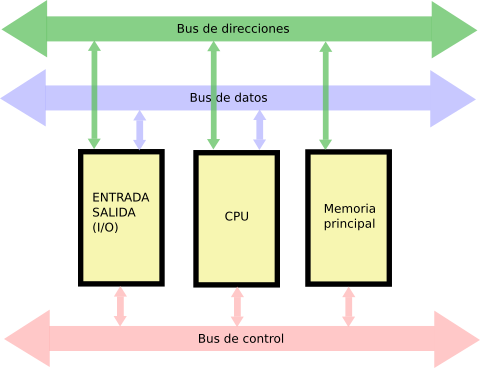
\includegraphics[scale=0.46]{buses-de-sistema.png}
    \caption{Unidades y buses del sistema}
\end{figure}

\subsection{Periféricos y Almacenamiento Externo}
Los \textbf{periféricos} son los dispositivos electrónicos, unidades externas, que se conectan al ordenador a través de los buses de entrada/salida, integrándose en el sistema, que pasa a controlarlos como parte de sí mismo desde el momento en el que se reconoce su conexión.

Existen infinidad de periféricos, diferentes por su diseño y función. Algunos tienen como finalidad facilitar la entrada de información en el ordenador, mientras que otros facilitan su salida, otros cuya finalidad es el almacenamiento permanente de datos o los que permiten la conexión con otras máquinas y el intercambio de información. No todos ellos son imprescindibles, aunque los más normal es contar de teclado, ratón, monitor, impresora altavoces y conexión de red.

Los periféricos se pueden clasificar, según su función, en los siguientes:

\begin{itemize}
    \item \textbf{Unidades de Entrada}: son aquellos periféricos que permiten introducir la información o los datos desde el exterior a la memoria principal, preparando la información para que pueda ser procesada por la máquina. Un ejemplo de estos periféricos son el teclado y el ratón.
    \item \textbf{Unidades de Salida}: son las encargadas de sacar al exterior los datos resultantes de las operaciones realizadas, mostrando la información de forma comprensible para el usuario. Ejemplos de estas unidades son la pantalla o la impresora.
    \item \textbf{Unidades de Entrada/Salida}: esta unidades de usan tanto para entrada como para la salida de información del sistema. Algunas de estas unidades no necesitan hacer procesos de conversión ya que manejan la información en formato binario, mientras que otras necesitan procesos de conversión para trabajar con los usuarios o para comunicarse con otro dispositivo. Algunos ejemplos son las tarjetas de red, discos duros, memorias USB, etc...
\end{itemize}

Algunos periféricos necesitan \textbf{soportes adicionales} para representar la información o almacenarla. En estos casos hay que tener en cuenta que el periférico no almacena la información, sino que es el medio utilizado para obtener o almacenar la información en su soporte. Un ejemplo de esto son los lectores de DVD o Blu-Ray.

\section{Componentes Físicos de un Ordenador Actual}
La arquitectura de un ordenador define la estructura funcional de cada una de sus partes, pero se hace necesario implementar dicha estructura mediante hardware de fabricación y comercialización actual. Dependiendo de  las características tecnológicas de los componentes empleados en su construcción (tamaño, grado de miniaturización, capacidad de procesado, ...), se ensamblarán ordenadores personales más o menos potentes, como portátiles, tablets, smartphones, consolas de juegos, etc... Pero también servidores, mainframes y superordenadores.

Hay que tener en cuenta, que los distintos componentes deben seguir unos estándares de fabricación, especialmente en lo relativo a sus conexiones y \textbf{\gls{interfaces}}, para permitir su completa integración con el sistema y mantener la compatibilidad de funcionamiento entre ellos.

En esta sección vamos a hacer un estudios de los diferentes elementos utilizados para el ensamblaje de un ordenador personal de sobremesa de uso general en base a componentes físicos que se fabrican y comercializan en la actualidad. Analizando en la medida de lo posible sus características de funcionamiento particulares.

\subsection{Cajas de Ordenador}
La \textbf{caja del ordenador}, también conocida como carcasa o chasis, es el ``recipiente'' donde se colocan todos los componentes del ordenador y que sirve para protegerlos. Estas cajas se fabrican en diversos materiales como acero, aluminio, plástico, metacrilato, etc.., o con una combinación de estos. Deben tener la suficiente resistencia para soportar el peso de los componentes en su interior, así como el calor que estos generan y suficiente espacio para albergarlos a todos con una distribución adecuada.

Estás cajas se fabrican siguiendo unos diseños de basados en unos \textbf{factores de forma} estándares, cada uno con sus propias características de tamaño, forma, capacidad, etc. Los principales factores de forma que nos podemos encontrar son los siguientes:

\begin{itemize}
    \item \textbf{Minitorre o Semitorre}: la diferencia entre ellas está en la altura y el número de \textbf{\gls{bahias}} de 5 y cuarto de que dispongan. A mayor número de bahías, más dispositivos podrá contener y más aumenta su altura. Suelen tener entre 2 y 4 bahías respectivamente.
    \item \textbf{Sobremesa}: son similares a las semitorres pero se colocan de forma horizontal, lo que obliga a rotar 90 grados los dispositivos extraíbles de su frontal.
    \item \textbf{Barebone y Slim}: son cajas de pequeño tamaño principalmente diseñadas para ocupar poco espacio. Esto implica que su interior admite pocos dispositivos, o ninguno, pero se compensa aumenta el número de conectores para dispositivos externos.
\end{itemize}

\begin{figure}[ht]
    \centering
    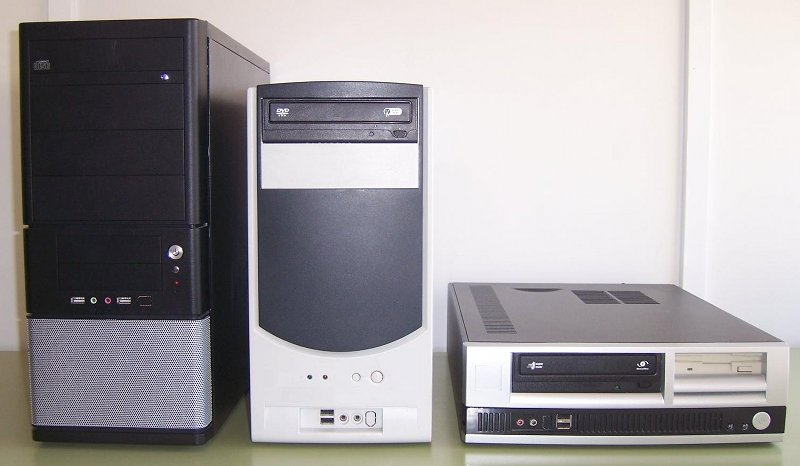
\includegraphics[scale=0.45]{torres-ordenador.jpg}
    \caption{Semitorre, Minitorre y Sobremesa}
\end{figure}

Para ampliar la información sobre los diferentes factores de forma que existen y las características de una caja de ordenador, podemos consultar \href{https://es.wikipedia.org/wiki/Caja_de_computadora}{esta entrada en Wikipedia}.

Independientemente del tamaño o forma que tenga que caja, hay ciertas características que deben tener para cumplir eficientemente su cometido:

\begin{itemize}
    \item En un interior, deben contener \textbf{diferentes compartimentos} dedicados a alojar la fuente de alimentación, los discos duros, las unidades ópticas y por supuesto, la placa base y las tarjetas de expansión que se conecten. En la siguiente figura podemos ver una imagen del interior de una caja (tipo semitorre), donde se pueden observar los diferentes compartimentos que posee.

    \item Deben tener un \textbf{panel frontal}, donde si sitúan los botones de encendido y reinicio, así como los LED que indican si el ordenador esta encendido y si se esta usando el disco duro.

    \item En el \textbf{panel trasero} se deben encontrar los diferentes conectores que vienen desde la placa base y las tarjetas de expansión, así como la toma de corriente.

    \item También deberá tener, distribuidas estratégicamente, \textbf{diferentes rejillas} que ayuden a la disipación del calor que generan los componentes en el interior de la caja.

   \begin{figure}[ht]
        \centering
        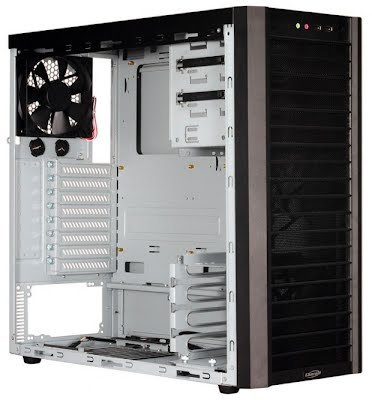
\includegraphics[scale=0.45]{caja-abierta.jpg}
        \caption{Caja de tipo semitorre abierta}
    \end{figure}
\end{itemize}

\subsubsection{Fuente de Alimentación}
La \textbf{fuente de alimentación} es una elemento imprescindible cuya misión es proporcionar corriente continua a todos los componentes que integran el interior de ordenador y a los de bajo consumo que se conectan externamente. Para ello debe de ser capa de suministrar un potencia no interior a 350 vatios. Hay que tener en cuenta que una fuente con potencia insuficiente puede causar mal funcionamiento y hasta dañar el equipo.

La fuente de alimentación suele venir preinstalada en la caja del ordenador, aunque no siempre es así, para poder elegir con independencia de la caja un modelo de fuente que se adapta de nuestras necesidades, por ejemplo, que tenga mayor potencia, más silenciosa, con más conectores de diferente tipo, etc...

Se suele presentar, como una caja pequeña, metálica, con muchas rejillas para ventilarse, de la que salen los cables con los \textbf{conectores} necesarios para alimentar los componentes del ordenador con voltajes de mas/menos \textbf{12 voltios}, \textbf{5 voltios} y más \textbf{3.3 voltios}. Los 12 voltios se suelen emplear para las unidades de almacenamiento y el ventilador, mientras que los 5 y 3.3 voltios para el resto de componentes.

Existen también fuentes de alimentación modulares que permiten el acoplamiento de los cables con los conectores necesarios, pudiendo retirar los cables sobrantes innecesarios para que no estorben dentro de la caja.

\begin{figure}[ht]
    \centering
    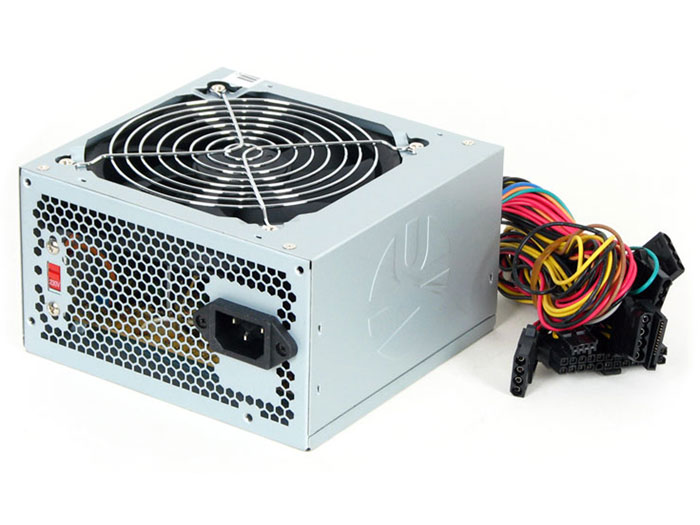
\includegraphics[scale=0.35]{fuente-alimentacion.jpg}
    \caption{Fuente de Alimentación}
\end{figure}

Desde la parte trasera de la fuente de alimentación podemos ver el conector para el cable de conexión a la fuente eléctrica y la rejilla de ventilación por la que su propio ventilador extrae el calor generado. Además, la parte trasera puede incluir, adicionalmente:

\begin{itemize}
    \item Un conector para la alimentación eléctrica del monitor.
    \item Un interruptor para el apaga total de la fuente de alimentación, que de otra forma permanece en estado de standby.
    \item Un selector para fijar la entrada de corriente alterna en 125 voltios o 220 voltios.
\end{itemize}

\subsection{Placas Bases}
La \textbf{Placa Base} es una tarjeta de circuito impreso donde se conectan el resto de componentes del computador. Contiene una serie de circuitos integrados entre los que se encuentra el \textbf{chipset}, que sirve como centro de conexión entre el procesador, la memoria RAM, los buses de expansión y otros dispositivos.

Su diseño debe cumplir con unos estándares basados en el \textbf{factor de forma}, que define algunas de las características físicas de esta, como por ejemplo:

\begin{itemize}
    \item La forma de la placa con sus dimensiones exactas (ancho y largo).
    \item La posición de los anclajes, es decir, donde se sitúan los tornillos para fijarla a la torre.
    \item Las áreas donde se sitúan algunos de sus componentes, como el zócalo del procesador, las ranuras de expansión y los conectores de la parte trasera.
    \item Las conexiones eléctricas de la fuente de alimentación: cantidad de conectores, forma, posición, etc...
\end{itemize}

En la siguiente imagen podemos ver una placa base con todos sus componentes.

\begin{figure}[ht]
    \centering
    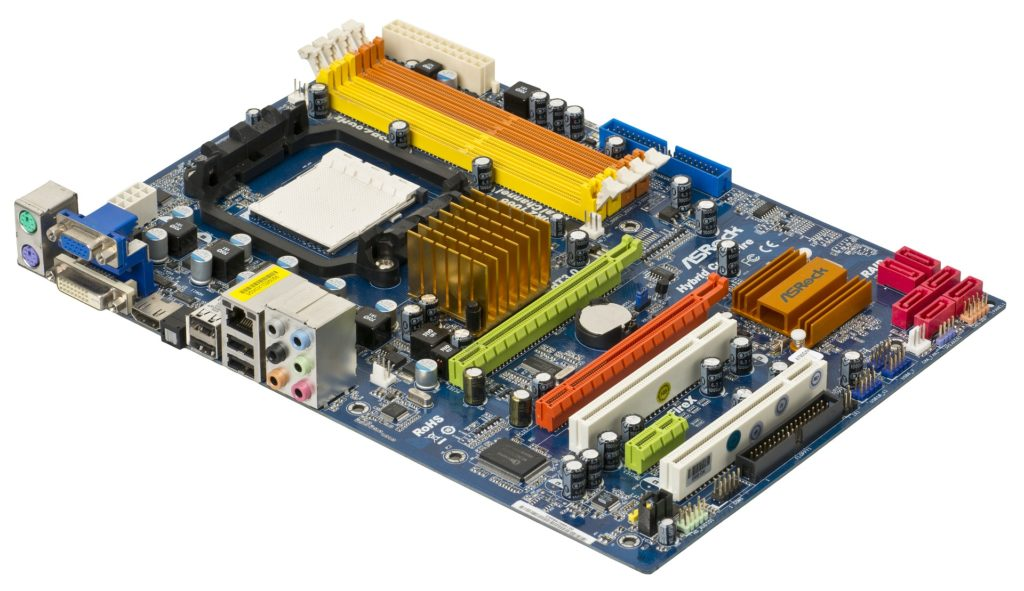
\includegraphics[scale=1]{placa-base.jpg}
    \caption{Placa base y sus componentes}
\end{figure}

Todos los conectores tienen conexión directa con alguno de los dos elementos principales del \textbf{chipset}, el \textbf{puente norte} o \textbf{northbridge} y el \textbf{puente sur} o \textbf{southbridge}. Se trata de dos circuitos integrados que con el tiempo han ido recogiendo en su diseño funcionalidades que antes fueron independientes. A saber:

\begin{itemize}
    \item \textbf{Northbridge}: se encarga de controlar funciones como las comunicaciones entre el procesador, la memoria y el sistema gráfico. Algunos modelos pueden incluir controladoras de vídeo, sonido y red.
    \item \textbf{Southbridge}: se encarga del control del resto de puertos internos y externos de la placa base.
\end{itemize}

\begin{figure}[ht]
    \centering
    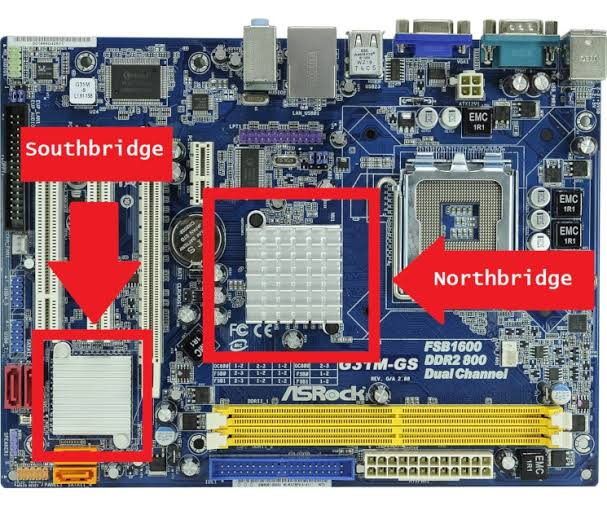
\includegraphics[scale=0.35]{puentes-placa.jpeg}
    \caption{Northbridge y Southbridge en una placa base}
\end{figure}

El chipset, por lo tanto, hace que la placa base funcione como un ``sistema nervioso'', que interconecta todos sus componentes por medio de diferentes buses, permitiendo la comunicación entre ellos.

La placa base también incluye un chip conocido como \textbf{\gls{BIOS}} con un software propio o \textbf{firmware}, que le permite realizar funcionalidades básicas, como reconocimiento y auto chequeo de los dispositivos instalados o gestión básica de vídeo y teclado. Es el software que se encarga del arranque del ordenador y que es independiente del sistema operativo.

En el \textbf{Anexo A.2} podemos encontrar una relación detallada de todos los componentes de una placa base, y que deberíamos de conocer.

\subsection{Procesadores}
El \textbf{procesador} es la parte más importante del computador ya que controla al resto de componentes. Se trata de un microchip compuesto de millones de microcomponentes recogidos en una cápsula, normalmente cerámica, que de la que salen una serie de patillas o contactos que hay que acoplar en el zócalo de la placa base.

Existen varios fabricantes de procesadores para ordenadores personales, siendo los mas potentes \textbf{AMD} e \textbf{Intel}, por ser los que más invierten en investigación y más productos sacan al mercado. En los siguientes enlaces podemos consultar los diferentes procesadores de estas compañías y su evolución.

\vspace{5ex}

\begin{itemize}
    \item \textbf{Procesadores AMD} - \url{http://www.configurarequipos.com/doc1043.html}
    \item \textbf{Procesadores Intel} - \url{http://www.configurarequipos.com/doc1051.html}
\end{itemize}

\begin{figure}[ht]
    \centering
    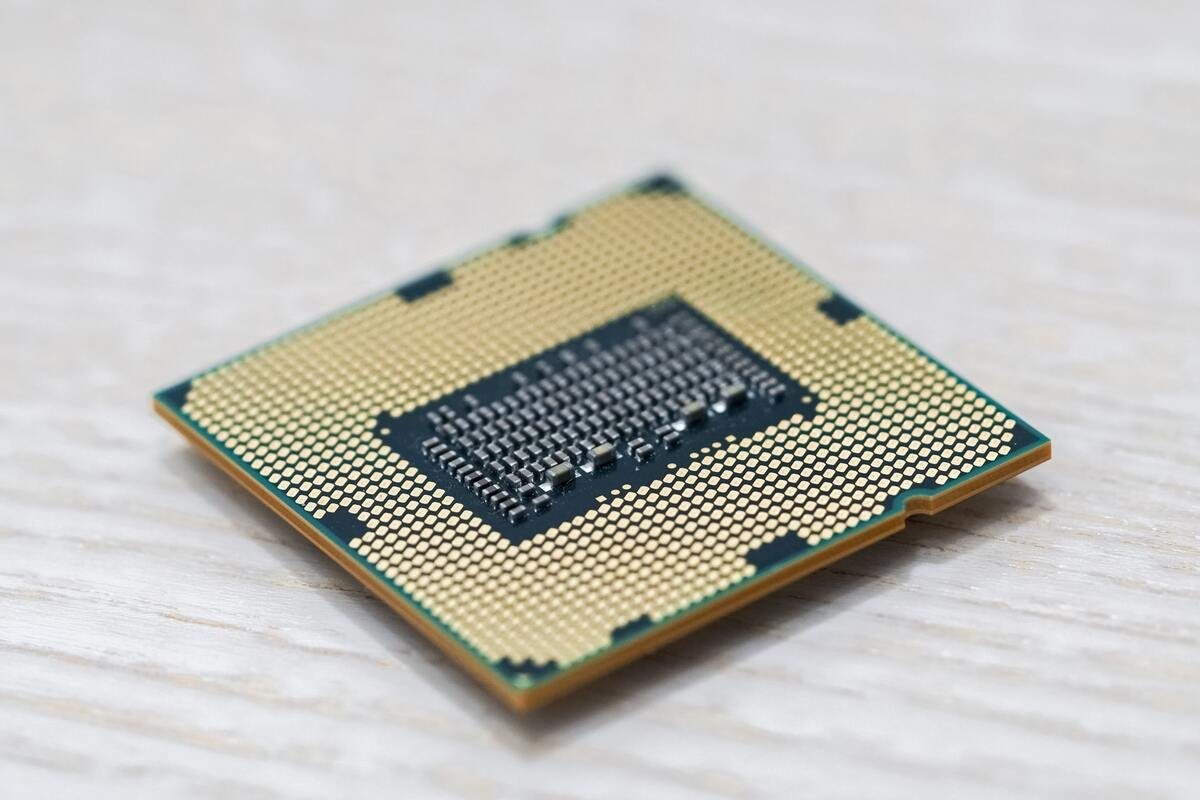
\includegraphics[scale=0.25]{cpu.jpg}
    \caption{Imagen de un procesador.}
\end{figure}

Hay diversas \textbf{características} que definen a un procesador:

\begin{itemize}
    \item \textbf{Velocidad de Cálculo}

    Es la velocidad de trabajo o frecuencia del reloj que me mide en \textbf{Hertzios}, o en alguno de sus submúltiplos. Con esta medida se especifica el número de ciclos por segundo, que esta relacionado con el número de operaciones por segundo que puede llevar a cabo el procesador. Se supone que cuantos mas hertzios tenga un procesador más operaciones podrá realizar por segundo y por lo tanto será más rápido.

    Hay que diferenciar entre al \textbf{velocidad interna} y la \textbf{velocidad externa} conocida como \textbf{Front Side Bus} (FSB), que es la velocidad de comunicación entre el procesador y la placa base. Esta medida es útil para comprar procesadores de un mismo fabricante, ya que ha iguales frecuencia de reloj pueden suponer diferentes velocidades de trabajo si comparamos procesadores de diferentes fabricantes.

    \item \textbf{Tecnología de Fabricación}

    La tecnología de fabricación, que se mide en \textbf{nanómetros}, es una medida utilizada para referirse al tamaño de los transistores que componen los procesadores. Cuanto menor sea el tamaño de los transistores, más cerca pueden colocarse unos de otros. Esto permite reducir la cantidad de energía eléctrica y por consiguiente reducir el calor generado por éstos durante el funcionamiento del microprocesador, que puede alcanzar mayores frecuencias de reloj. Actualmente se están fabricando procesadores entre 32 nm y 12 nm.

    \item \textbf{Tamaño y Nivel de la Memoria Caché}

    Es una memoria de gran velocidad utilizada para almacenar datos e instrucciones a los que el procesador debe de estar accediendo continuamente. La inclusión de una buena cantidad de memoria caché aumenta el rendimiento ya que permite reducir el número de accesos que se realizan a la memoria RAM, más lenta.

    Suele haber varios tipos de memoria caché que se \textbf{organizan por niveles}, creando una jerarquía basada en en la proximidad al núcleo del procesador, de forma que cuanto más cerca éste, trabajará a mayor velocidad, pero será de menor tamaño. La cache puede ser:

    \begin{itemize}
        \item \textbf{Caché de primer nivel o L1}: caché que esta integrada en el núcleo del procesador y trabaja a la misma velocidad. Su capacidad varía de un procesador a otro estando entre los 64KB y los 512KB. Suele estar dividida en dos parte, una dedicada a trabajar con los datos y otra con las instrucciones.

        \item \textbf{Caché de segundo nivel o L2 y tercer nivel o L3}: suelen estar también integradas en el procesador aunque no en su núcleo y sus tamaños pueden variar entre los 3 MB y los 6 MB.
    \end{itemize}

    \item \textbf{Número de Núcleos}

    Otra de la características de los procesadores actuales es el \textbf{número de núcleos} que se integra en la cápsula y que pueden trabajar de forma simultánea. Como se esta haciendo difícil, o poco rentable, incrementar la velocidad de funcionamiento de los nuevos procesadores para continuar aumentando su rendimiento, los fabricantes han aprovechado el alto grado de integración conseguido en la fabricación de estos para encapsular varios núcleos dentro de un mismo procesador. Actualmente podemos encontrar procesadores con un variable número de núcleos, desde 2 núcleos a 16, o incluso más.

    \item \textbf{Arquitectura}

    En relación al funcionamiento, cabe destacar que otra característica de los procesadores es su \textbf{arquitectura}, la cual puede ser de \textbf{32 bits} o \textbf{64 bits}, que son los tamaños más utilizados en la actualidad. Esta medida se refiere al tamaño de los registros que contiene el procesador, y por tanto, al tamaño de las instrucciones que puede procesar éste. De este tamaño, dependerá el resto de la arquitectura del resto de componentes del procesador, ya que tendrán que trabajar con el mismo número de bits.
\end{itemize}

Hay que tener en cuenta que la elección de un procesador \textbf{condiciona la elección} de la \textbf{placa base}, ya que debe incluir un chipset acorde para que se puedan aprovechar todas las características del procesador, así como un zócalo compatible en el que pueda instalarse.

Además, hay que tener en cuenta que los procesadores, durante su funcionamiento, generan una gran cantidad de calor, por lo que deberemos tener en cuenta la incorporación de algún \textbf{sistema de refrigeración} que ayude a lidiar con el este calor. Los disipadores, que suelen ser los más empleados, consisten en un elemento metálico (de aluminio o cobre), con mucha superficie de contacto con el aire, que absorba el calor del procesador disipándolo en el aire. Esta \textbf{disipación} puede ser de dos tipos:

\begin{itemize}
    \item \textbf{Disipación pasiva}: solo incluye el disipador, el elemento metálico ya mencionado.
    \item \textbf{Disipación activa}: además del disipador, incluye un ventilador acoplado al disipador que crea un flujo de aire ayudando a disipar el calor más rápidamente.
\end{itemize}

Además, existen alternativas como por ejemplo la \textbf{refrigeración líquida}, que extrae el calor del procesador y de otros componentes aprovechando su mayor conductividad, aunque tiene el inconveniente de tener que instalar circuitos cerrados para hacer pasar el líquido por las zonas a refrigerar además de necesitar un radiador externo para que el líquido se desprenda de su calor.

\subsection{Memorias RAM}
La \textbf{memoria de acceso aleatorio} o memoria RAM (Random Access Memory) es la memoria que necesita el procesador para ejecutar los programas. En ella busca las instrucciones y datos, además de almacenar los resultados de las operaciones realizadas.

Físicamente, las memorias RAM son pequeñas tarjetas de circuito impreso en la que se sueldan los chips de memoria, por una o ambas caras. Llevan en uno de sus cantos un conjunto de pines o contactos metálicos para insertarlas en los zócalos de la placa base.

\begin{figure}[ht]
    \centering
    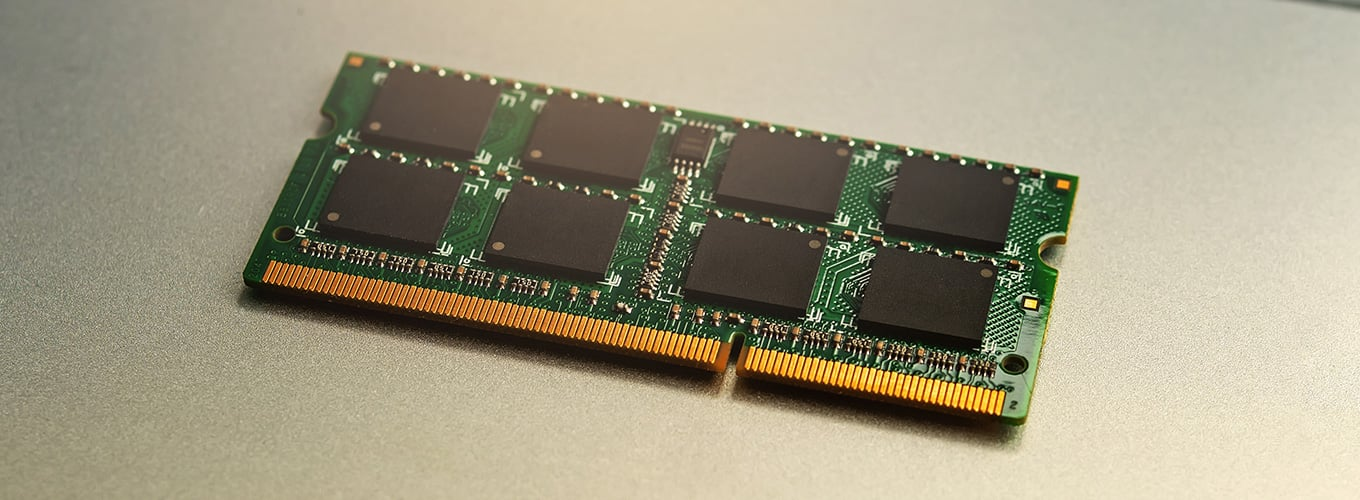
\includegraphics[scale=0.25]{ram.jpg}
    \caption{Módulo de memoria RAM tipo SO-DIMM}
\end{figure}

Actualmente podemos encontrar en el mercado diferentes tipos de módulos RAM, los más usados son de tipo \textbf{DDR} (Double Data Rate) o doble tasa de transferencia de datos que vienen integrados en tarjetas de memoria de tipo \textbf{DIMM} o \textbf{SO-DIMM}, usados en equipos de sobremesa y portátiles respectivamente.

Dentro de los módulos DDR, podemos encontrar diferentes versiones que determinarán el número de pines que poseen y donde se encuentra la muesca que les impide su colocación de forma incorrecta. Los principales tipos son:

\begin{itemize}
    \item \textbf{DDR}: son módulos RAM que usan memorias síncronas (SDRAM), en encapsulados de tipo DIMM, y que permiten hacer \textbf{dos transferencias simultáneas} en un mismo ciclo de reloj. Tienen \textbf{184 pines} en DIMM y \textbf{200 pines} en SO-DIMM.

    \item \textbf{DDR2}: trabajan al doble de frecuencia del reloj de la memoria, por lo que durante cada ciclo de reloj se realizan \textbf{cuatro trasferencias}. Tienen \textbf{240 pines} en DIMM y \textbf{200 pines} en SO-DIMM.

    \item \textbf{DDR3}: pueden realizar\textbf{ ocho transferencias }de datos por cada ciclo de reloj. Tiene \textbf{240 pines} en DIMM y \textbf{204 pines} en SO-DIMM.

    \item \textbf{DDR4}: no aumenta el número de transferencias de reloj, manteniéndose en 8, pero \textbf{aumenta la velocidad} incrementando la frecuencia de reloj. Además, tienen \textbf{mayor densidad} (mayor capacidad de datos) y menores requisitos de voltaje. Usan encapsulados DIMM con \textbf{288 pines} y SO-DIMM con \textbf{260 pines}.
\end{itemize}

\subsection{Tarjetas de Vídeo}
Una \textbf{tarjeta de vídeo} o \textbf{tarjeta gráfica}, es una tarjeta de expansión adicional, que adapta los daros enviados por el procesador al monitor o proyector para que el usuario pueda verlos representados.

La conexión de estos adaptadores a la placa base se realiza a través del bus \textbf{PCI Express x16}, ya que necesitan un bus rápido de comunicaciones. Hay modelos de  placas base y procesadores que integran en su circuitería un controlador gráfico de suficiente calidad para el uso normal del ordenador, pero que queda escaso de potencia de trabajo para aplicaciones que hagan uso intensivo de representación gráfica, como juegos o modelado 3D.

Para satisfacer la necesidades superiores gráficas de algunos programas, de diseño o juegos, hay placas base que ofrecen la posibilidad de conectar más de una tarjeta gráfica de modo que éstas puedan trabajar como una sola aumentando considerablemente su potencia.

\begin{figure}[ht]
    \centering
    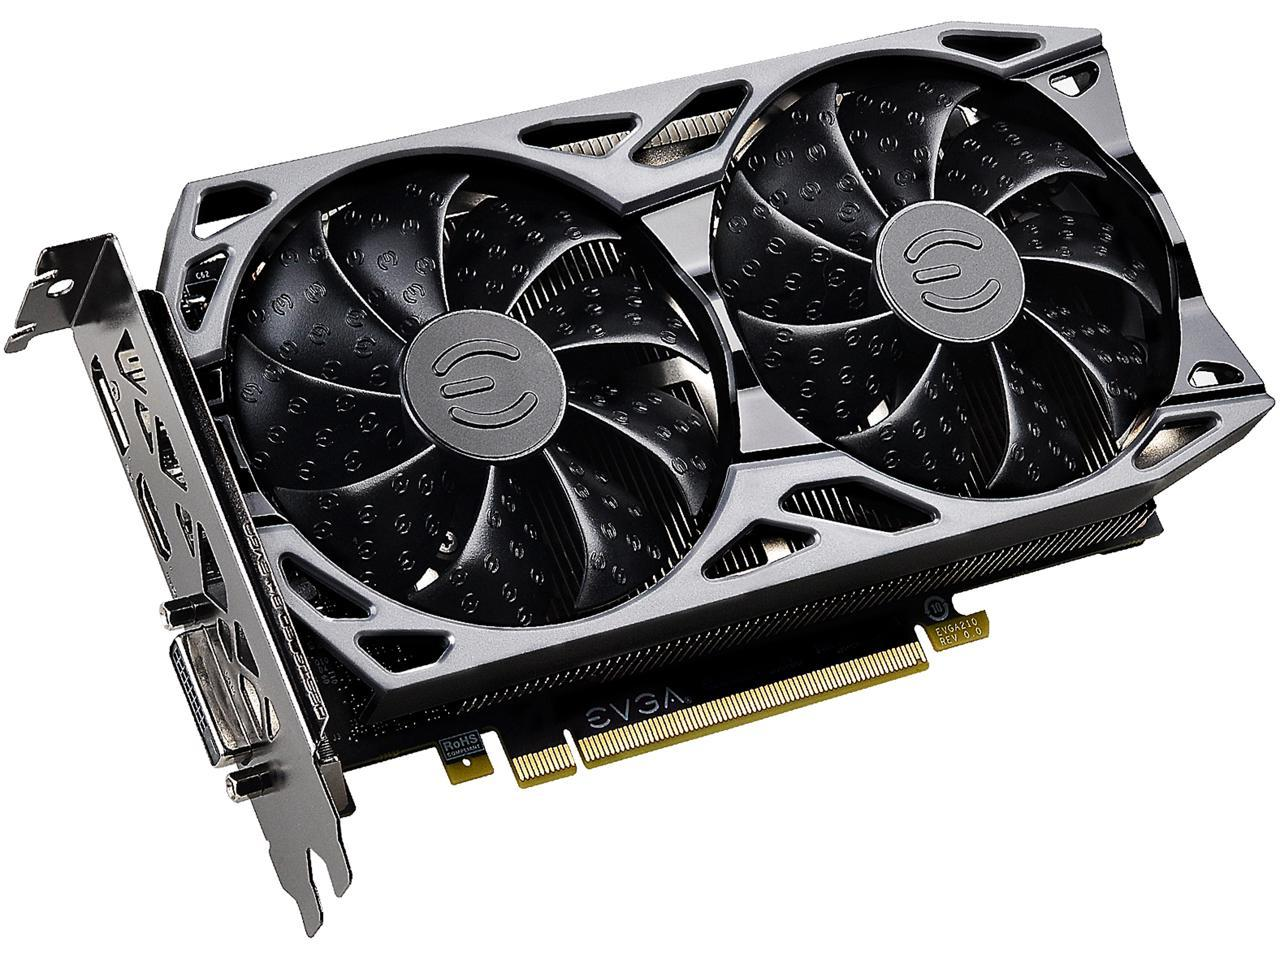
\includegraphics[scale=0.18]{gpu.jpg}
    \caption{Tarjeta gráfica con disipación activa}
\end{figure}

\newpage

Las tarjetas gráficas suelen tener, como mínimo, los siguientes elementos:

\begin{itemize}
    \item \textbf{La GPU}: es un procesador dedicado en exclusiva al tratamiento de gráficos, que libera al procesador de esta tarea. Necesita, al igual que el procesador, sistemas de refrigeración para disipar el calor.

    \item \textbf{La Memoria}: memoria que incorporan para el uso exclusivo de la propia tarjeta. Se llama memoria de vídeo y suele ser incluso más eficiente que la RAM del computador. Cuando la tarjeta gráfica esta integrada en la placa base o el procesador se suele reservar una parte de la memoria RAM para el uso de ésta.

    \item \textbf{EL RAMDAC}: es un conversor de imagen digital a analógica. Su función es transformar las señales para que pueden ser reproducidas en monitores analógicos. Este componente desaparece cuando todos los monitores sean digitales y reproduzcan directamente la señal digital.
\end{itemize}

Además de estos elementos, las tarjetas gráficas suelen incluir diferentes \textbf{conexiones} entre la tarjeta y ek monitor, siendo las más comunes son, \textbf{\gls{DVI}}, \textbf{\gls{S-Video}}, \textbf{\gls{SVGA}} y \textbf{\gls{HDMI}}.

Para ampliar más información sobre las tarjetas gráficas, podemos visitar su \href{https://es.wikipedia.org/wiki/Tarjeta_gr\%C3\%A1fica}{entrada en Wikipedia.}

\subsection{Tarjetas de Sonido}
Una \textbf{tarjeta de sonido} es una tarjeta de expansión que permite la entrada y salida de audio a través de sus conectores. Normalmente se inserta en una ranura \textbf{PCI}, aunque la mayoría de modelos de placa base vienen ya con una integrada. Las tarjetas de sonido incorporan conectores de tipo mini-jack que se necesitan para la conexión de equipos de sonido. Estos conectores tienen un código de colores que detallamos a continuación:

\begin{itemize}
    \item Entrada analógica para micrófono: \textbf{rosa}.
    \item Entrada analógica ``Line-In'': \textbf{azul}.
    \item Salida analógica estéreo para altavoces frontales: \textbf{verde}.
    \item Salida analógica para altavoces traseros: \textbf{negro}.
    \item Salida analógica para altavoces laterales: \textbf{plateado}.
    \item Salida digital SPDIF: \textbf{naranja}.
\end{itemize}

Además de estas conexiones, algunas tarjetas incluyen una

\begin{figure}[ht]
    \centering
    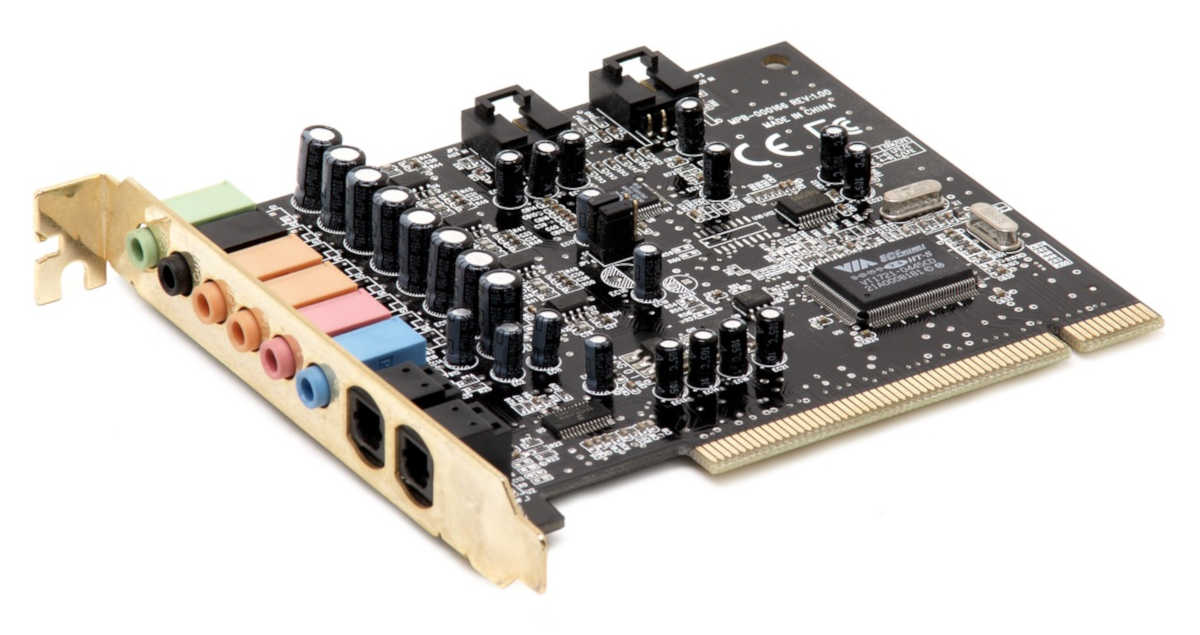
\includegraphics[scale=0.25]{tarjeta-sonido.jpg}
    \caption{Tarjeta de sonido}
\end{figure}

Las tarjetas de sonido necesitan tener varios componentes para poder procesar el sonido. Estos componentes son los siguientes:

\begin{itemize}
    \item \textbf{Circuito CAD} (Conversor Analógico-Digital): se encarga de transformar la señal analógica del sonido en su equivalente digital.
    \item \textbf{Circuito DAC} (Conversor Digital-Analógico): se encarga de transformar la señal digital en analógica de modo que pueda ser reproducida en unos altavoces.

    Para que la tarjeta de sonido pueda grabar y reproducir sonido al mismo tiempo ambos conversores, el CAD y el DAC, deben trabajar de forma independiente, lo que se conoce como \textbf{full-duplex}.

    \item \textbf{Circuito DSP} (Procesador de Señal Digital): se encarga de procesar el audio en su forma digital, realizando la compresión del audio cuando se graba y descomprimiendo cuando se reproduce. Además, por medio de algoritmos puede aplicar efectos acústicos  a los sonidos como coros, reverb, etc...

    \item \textbf{Sintetizador FM} (Modulación de Frecuencia): se encarga de generar sonido en formato \textbf{\gls{MIDI}} a partir de representaciones simbólicas de sus características.

    \item \textbf{Sintetizador por Tablas de Onda}: genera el sonido a partir de conjunto de muestras de sonido, de instrumentos reales, pregrabados en formato digital en una memoria ROM que incluye la propia tarjeta. El sintetizador para reproducir audio busca en las tablas que necesita en cada momento.

    \item \textbf{Mezclador}: tiene como finalidad recibir múltiples entradas, combinarlas adecuadamente, y enviarlas a las salidas.
\end{itemize}

Para obtener más información sobre las tarjetas de sonido, podemos visitar la \href{https://es.wikipedia.org/wiki/Tarjeta_de_sonido}{entrada en Wikipedia} referente a éstas.

\subsection{Dispositivos de Entrada}
Son todos aquellos \textbf{periféricos} que puede utilizar el usuario para \textbf{introducir información} al ordenador. Para ello será necesario que estén conectados a éste de alguna de las formas posibles. La mayoría de conexiones utilizadas, sobre todo en dispositivos de bajo consumo, reciben la alimentación necesaria a través del mismo conector, como por ejemplo, el teclado o el ratón. En cambio, otros dispositivos, debido a su alto consumo, necesitarán tener su propia fuente de alimentación, como por ejemplo, algunos escáneres. A continuación mostramos una lista con los dispositivos de entrada más comunes que nos podemos encontrar.

\begin{itemize}
    \item \textbf{Teclado}

    Es uno de los dispositivos de entrada más comunes, y casi imprescindibles, que utilizamos para \textbf{enviar información} al ordenador mediante la \textbf{pulsación de sus teclas}. Su modo de funcionamiento incluye que lo tecleado aparezca automáticamente en la pantalla, pudiendo así comprobar que se ha teclado de forma correcta.

    Se conecta al ordenador mediante un conector de tipo \textbf{PS/2} (o mini-din) a su conexión exclusiva, o por medio de conector \textbf{USB}. También los hay \textbf{inalámbricos} que necesitan dos terminales con emisor y receptor, uno de ellos en el propio teclado y otro que debe estar conectado al ordenador mediante el puerto PS/2 o USB. Además, entre los inalámbricos nos encontramos a los que usan el protocolo \textbf{bluetooth}, pudiendo aprovechar los emisores ya incorporados al ordenador.

    \begin{figure}[ht]
        \centering
        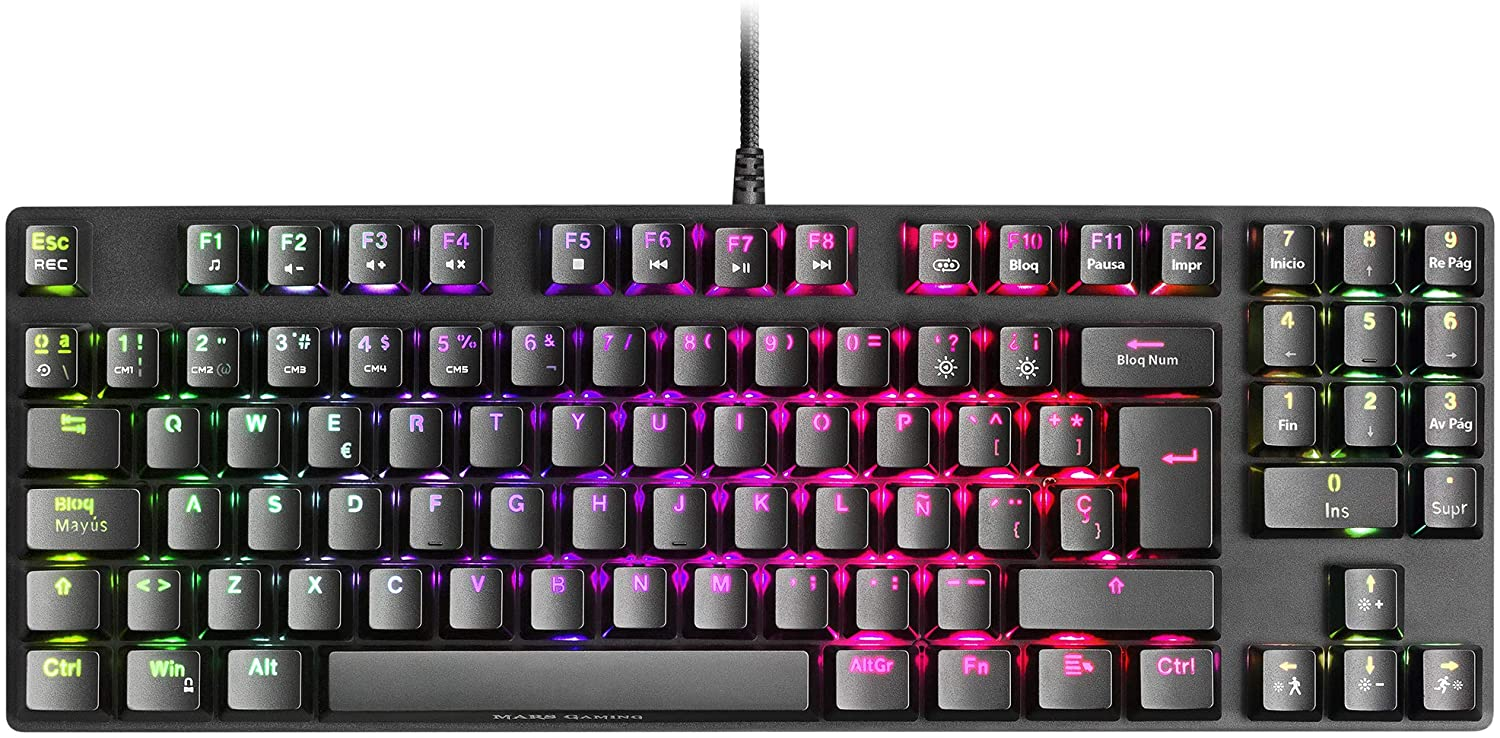
\includegraphics[scale=0.15]{teclado.jpg}
        \caption{Teclado estándar}
    \end{figure}

    \item \textbf{Ratón}

    El teclado es un dispositivo que al \textbf{ser desplazado} por una superficie plana, \textbf{mueve} sobre la pantalla un \textbf{cursor} que lo representa reflejando sus movimientos.

    Dependiendo del modelo, el ratón puede tener dos o más botones, incluso varias ruedas de desplazamiento, que permiten dar diversas órdenes en función del botón pulsado y del número de pulsaciones.  El cursor, que suele tener forma de flechas, se usa para \textbf{señalar diferentes objetos gráficos} en la \textbf{pantalla}.

    Se conecta al ordenador mediante un puerto PS/2 o USB, aunque al igual que con los teclados, podemos encontrarlos inalámbricos.

    \vspace{4ex}

    \begin{figure}[ht]
        \centering
        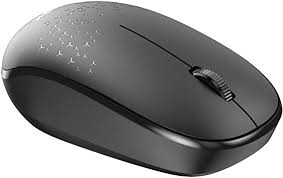
\includegraphics[scale=0.50]{raton.jpg}
        \caption{Ratón con 2 botones y rueda}
    \end{figure}


    \item \textbf{Joystick}

    El joystick o palanca es un periférico similar al ratón en cuanto \textbf{transmite los movimientos} que realicemos con él al ordenador. Se  utiliza sobre todo en juegos para dirigir el movimiento de personajes o vehículos.

    Suele conectar el ordenador mediante un puerto USB. Algunas tarjetas de sonido traen un conector específico para él.

    \begin{figure}[ht]
        \centering
        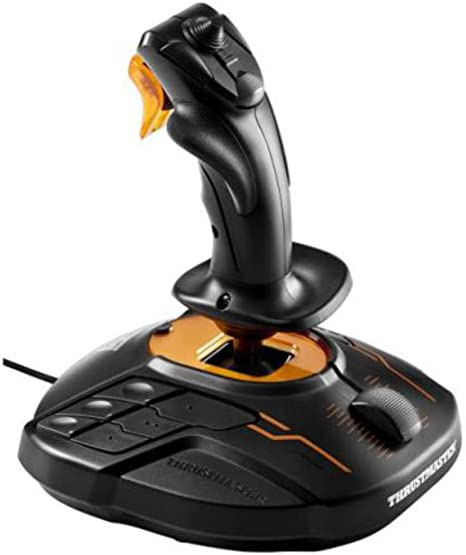
\includegraphics[scale=0.25]{joystick.jpg}
        \caption{Joystick estándar}
    \end{figure}

    \item \textbf{Escáner}

    Se utiliza para \textbf{explorar objetos} y obtener su \textbf{representación digital}. El proceso de digitalización consiste en tomar información de cada punto de la superficie del objeto y representarlos con valores binarios para generar un duplicado digital que pueda procesador el ordenador.

    Utiliza una conexión USB para conectarse al ordenador y algunos necesitan toma de corriente eléctrica para su propia alimentación. Además, podemos encontrar diferentes modelos de escáner,  como de sobremesa, de rodillo, de tambor, etc...

    \begin{figure}[ht]
        \centering
        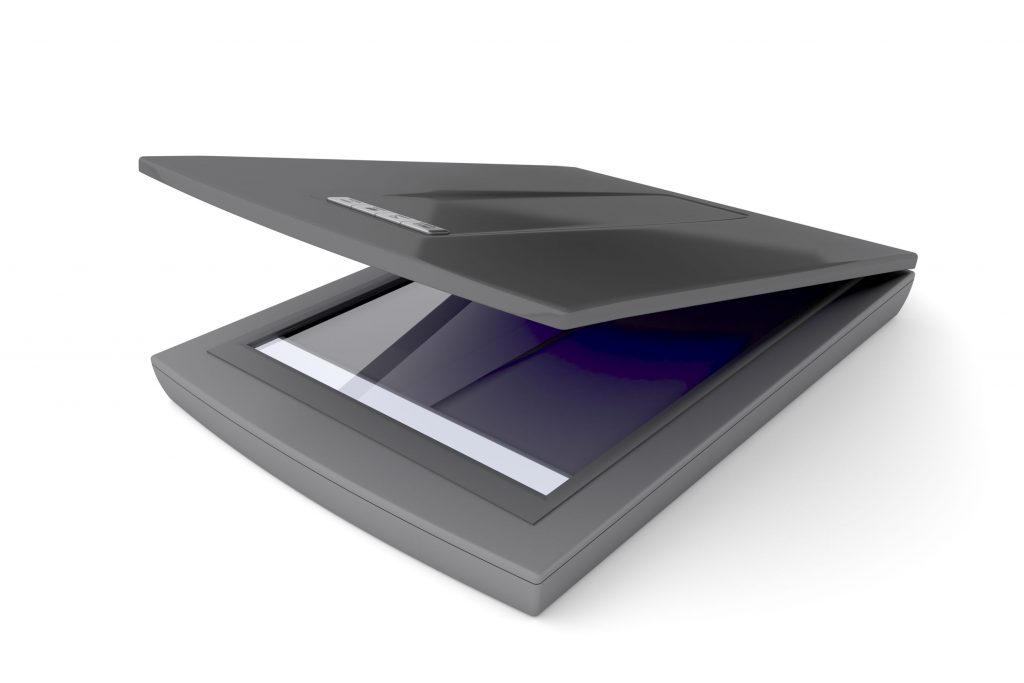
\includegraphics[scale=0.30]{escaner.jpg}
        \caption{Escáner de sobremesa}
    \end{figure}

    \item \textbf{Lectores de Código de Barras}

    Podemos encontrar tanto lectores de mano como fijos. Ambos, son \textbf{escáneres especializados} en la tarea de leer e interpretar códigos de barras. No se utilizan para obtener la representación digital del código de barras, sino el valor numérico que representan. Según el modelo, pueden conectarse al ordenador por USB, puerto de serie, Wi-Fi, bluetooth e incluso al puerto del teclado medio de un adaptador.

     \begin{figure}[ht]
        \centering
        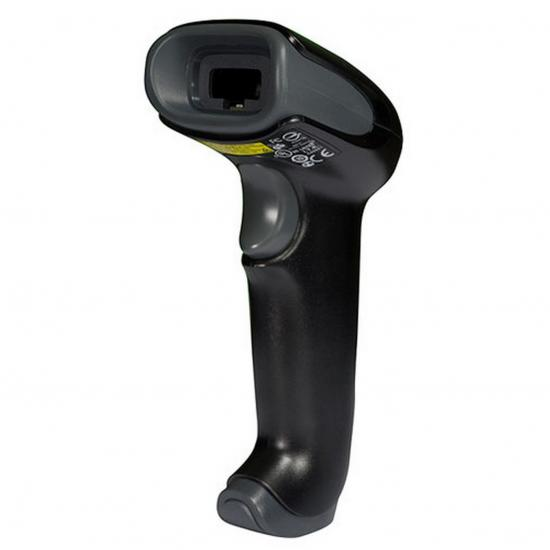
\includegraphics[scale=0.25]{lector-barras.jpg}
        \caption{Lector de código de barras de mano}
    \end{figure}

    \item \textbf{Tableta Gráfica o Digitalizadora}

    Este periférico permite la \textbf{introducción de dibujos o gráficos} dibujados \textbf{a mano} como si se hiciera con papel y lápiz. Se trata de una tablilla plana donde el usuario escribe utilizan el lápiz que suele acompañarla, aunque los trazos aparecen en la pantalla en vez de en la tableta.

    Algunas tabletas tiene delimitadas zonas de actuación que al ser pulsadas con el lápiz funcionan como botones e incluso pueden usarse como un ratón de gran precisión ya que permite apuntar y seleccionar los objetos que se encuentran en pantalla. Las tabletas actuales, suelen conectarse mediante el puerto USB, aunque hay modelos que lo hacen mediante bluetooth o Wi-Fi.

    \begin{figure}[ht]
        \centering
        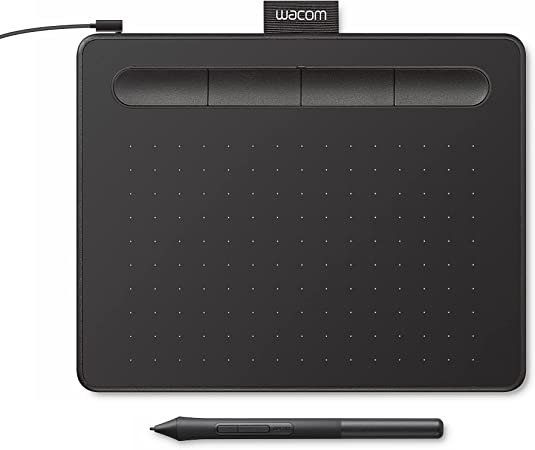
\includegraphics[scale=0.32]{tableta-digi.jpg}
        \caption{Tableta digitalizadora y su lápiz}
    \end{figure}

    \item  \textbf{Micrófono}
\end{itemize}











% Glossary

\glsaddall
\printglossaries

% Bibliography

\newpage
\addcontentsline{toc}{chapter}{Bibliografía}
\bibliography{citas}
\bibliographystyle{unsrt}

\end{document}